% !TEX root = ../main.tex
This thesis asks how many connections a network can have before some pair of points has too many independent routes between them. This chapter defines the problem and its variants, and states the results that are proved.

\section{Graphs and routes}

A \emph{multigraph} $G$ consists of a finite set $V(G)$ of \emph{vertices} and a multiset $E(G)$ of \emph{edges}. Each edge joins two different vertices, and edges can have identical copies. 
The number of such identical edges between $u$ and $v$ is the multiplicity $\mu(u,v)$.
If $\mu(u,v)\le1$ for every pair, then $G$ is a \emph{simple graph}.
The \emph{size} of $G$ is its number of edges, counted with multiplicity: $|E(G)|=\sum_{\{u,v\}}\mu(u,v)$.
This thesis tries to maximize the size.
Drawing vertices as dots and edges as lines is the standard way to visualize graphs.

\begin{figure}[ht]
\centering
\begin{tikzpicture}[scale=1.0,
    mv/.style={gvertex},
    me/.style={gline}]
  \foreach \i in {0,...,4} {
    \pgfmathsetmacro{\ang}{90 + 72*\i}
    \coordinate (v\i) at (\ang:1.4);
  }
  \draw[me] (v0)--(v1) (v0)--(v2) (v0)--(v3)
            (v1)--(v2) (v1)--(v4)
            (v2)--(v3) (v2)--(v4)
            (v3)--(v4);
  \foreach \i in {0,...,4} {
    \pgfmathsetmacro{\ang}{90 + 72*\i}
    \node[mv] at (\ang:1.4) {$\i$};
  }
\end{tikzpicture}
\caption{The simple graph $K_5-\{04,13\}$ has five vertices and eight edges, where $K_n$ is the complete graph on $n$ vertices.}
\label{fig:k5-example}
\end{figure}

We write $n\coloneq|V(G)|$. The \emph{degree} of a vertex is the number of edges at it.
From now on, graphs are simple unless we say otherwise.
A \emph{path} from $u$ to $v$ is a sequence $v_0,e_1,v_1,\ldots,e_q,v_q$ of distinct vertices $v_i$ and edges $e_i$, where $v_0=u$, $v_q=v$ and $e_i$ joins $v_{i-1}$ and $v_i$.
In a multigraph, two parallel edges give two different paths of length one.
In a simple graph we can write a path as a list of vertices.
A graph is \emph{connected} if every two vertices are joined by a path. A \emph{tree} is a connected graph in which every two vertices are joined by exactly one path. A tree on $n$ vertices has $n-1$ edges \cite{Diestel17}. A \emph{forest} is a graph without cycles. A \emph{spanning tree} of a graph $G$ is a tree on all vertices of $G$ that uses only edges of $G$.
Two $u$--$v$ paths are \emph{edge-disjoint} if they have no edge in common.
The \emph{local edge-connectivity} $\lec_G(u,v)$ is the largest number of pairwise edge-disjoint $u$--$v$ paths.
Its largest value over all pairs is
\[
    \lec_G^{\max} = \max_{u \ne v} \lec_G(u, v).
\]
If $G$ has fewer than two vertices, we set $\lec_G^{\max}=0$.
\begin{theorem}[Menger \cite{Menger27,FordFulkerson56}]\label{thm:menger-main}
Let $u$ and $v$ be distinct vertices of a multigraph $G$. The largest number of pairwise edge-disjoint $u$--$v$ paths equals the smallest number of edges whose removal leaves no $u$--$v$ path.
\end{theorem}
\Cref{fig:menger} shows an example.

\begin{figure}[ht]
\centering
\begin{tikzpicture}[scale=1.2,
    mv/.style={gvertex},
    me/.style={gline},
    rA/.style={grA},
    rB/.style={grB},
    rC/.style={grC},
    cut/.style={gcutedge}]
  \foreach \i in {0,...,4} {
    \pgfmathsetmacro{\ang}{90 + 72*\i}
    \coordinate (v\i) at (\ang:1.5);
  }
  % all eight edges, faint background
  \draw[me] (v0)--(v1) (v0)--(v2) (v0)--(v3)
            (v1)--(v2) (v1)--(v4)
            (v2)--(v3) (v2)--(v4)
            (v3)--(v4);
  % three edge-disjoint routes between the non-adjacent pair 1 and 3
  \draw[rA] (v1)--(v0)--(v3);
  \draw[rB] (v1)--(v2)--(v3);
  \draw[rC] (v1)--(v4)--(v3);
  % minimum cut: the three edges meeting vertex 1, a dashed ring around it
  \draw[cut] (v1) circle (0.6);
  \node[vertexred, font=\scriptsize] at (-1.35,1.55) {cut: $3$ edges};
  \foreach \i in {0,...,4} {
    \pgfmathsetmacro{\ang}{90 + 72*\i}
    \node[mv] at (\ang:1.5) {$\i$};
  }
\end{tikzpicture}
\caption{Menger's theorem on \Cref{fig:k5-example}: three edge-disjoint $1$--$3$ routes (coloured) meet the minimum three-edge cut around vertex $1$, so $\lec(1,3)=3$.}
\label{fig:menger}
\end{figure}

\section{Erd\H{o}s Problem 915}

Fix an integer $m\ge2$.
The condition $\lec_G^{\max}\le m-1$ means that no two vertices are joined by $m$ edge-disjoint paths.
By Menger's theorem, it also means that any two vertices can be separated by removing at most $m-1$ edges.
We ask how many edges a graph can have under this condition.

\begin{ques}[Erd\H{o}s Problem 915 \cite{ErdosProblems}]
How many edges can a graph on $n$ vertices have if no two of its vertices are joined by $m$ disjoint paths?
\end{ques}

The database \cite{ErdosProblems} notes that the original statement leaves open whether ``disjoint'' means edge-disjoint or internally vertex-disjoint.
This thesis takes edge-disjoint paths as the main question and treats vertex-disjoint paths as a variant (\Cref{sec:variants}).

We write
\[
    \ell_m(n) = \max\{\, |E(G)| : |V(G)| = n,\ \lec_G^{\max} \le m - 1 \,\}
\]
for the answer.
Mader proved the following upper bound where $\floor{x}$ is $x$ rounded down and $\ceil{x}$ is $x$ rounded up.

\begin{theorem}[Mader \cite{Mader73}]\label{thm:mader}
For all $n \ge 2$ and $m \ge 2$,
\[
    \ell_m(n) \le \floorfrac{m(n-1)}{2}.
\]
\end{theorem}

Bollob\'{a}s and Erd\H{o}s \cite{BollobasErdos62} found graphs that attain this bound when $m-1$ divides $n-1$: copies of $K_m$ that share one vertex.
For $n\ge m$ the bound is always attained (\Cref{thm:extremal-existence}).
For $2\le n<m$ the complete graph $K_n$ satisfies the condition, so $\ell_m(n)=\binom n2$.
This is smaller than $\floor{m(n-1)/2}$, except when $(n,m)=(2,3)$.

\Cref{sec:mader-gomory-hu} proves \Cref{thm:mader} in a different way from Mader, with the Gomory--Hu tree.
This is a tree on the vertices of $G$ with a weight on each edge.
For every pair $u,v$, the value $\lec_G(u,v)$ is the smallest weight on the path from $u$ to $v$ in the tree.
So the $\binom n2$ values $\lec_G(u,v)$ are stored in only $n-1$ weights.
The edges of the tree need not be edges of $G$.
The proof counts the edges of $G$ in two ways with this tree.
The same method proves the bound for multigraphs (\Cref{thm:multigraph-edge}).


\section{Variants of the problem}\label{sec:variants}

We change four assumptions. The first three give eight graph models.
In each model we can ask for edge-disjoint or for vertex-disjoint routes (\Cref{sec:incidence-convention}).

The first assumption is the size of an edge.
A \emph{hyperedge} is a set of $r\ge2$ vertices.
In an \emph{$r$-uniform hypergraph} every hyperedge has exactly $r$ vertices.
A \emph{Berge path} is a sequence of distinct vertices and distinct hyperedges, alternating, in which each hyperedge contains the vertex before it and the vertex after it.
This aligns best with the path definition for multigraphs.
The size of a hypergraph is its number of hyperedges, counted with multiplicity.

The second assumption is repetition.
A \emph{simple} graph or hypergraph has each edge at most once.
A \emph{multigraph} or \emph{multihypergraph} may repeat edges.

The third assumption is direction.
A directed edge, or \emph{arc}, is an ordered pair of vertices.
A directed hyperedge has one \emph{tail} and $r-1$ \emph{heads}.
A directed Berge route enters a hyperedge at its tail and leaves it at a head.
In the figures, one colour is one hyperedge, not a path of ordinary edges.
\Cref{fig:eight-models} shows the eight models.

\begin{figure}[ht]
\centering
\resizebox{\textwidth}{!}{%
\begin{tikzpicture}[>=Stealth,
    mv/.style={gvertex, minimum size=5.5mm},
    me/.style={gline},
    ml/.style={metro, line width=2.8pt},
    stn/.style={metrostop, minimum size=5mm},
    darc/.style={gdir},
    hstar/.style={metro, line width=2.7pt, -{Stealth[length=2.8mm]}, shorten >=3.2mm, shorten <=2.4mm}]
  % (a) simple graph: K_3 triangle, single edges only
  \begin{scope}[shift={(0,0)}]
    \node[mv] (s1) at (90:0.78) {};
    \node[mv] (s2) at (210:0.78) {};
    \node[mv] (s3) at (330:0.78) {};
    \draw[me] (s1)--(s2)  (s2)--(s3)  (s3)--(s1);
    \node[font=\itshape] at (0,-1.75) {simple graph};
    \node[font=\scriptsize, text=black!65] at (0,-2.25) {one edge per pair};
  \end{scope}
  % (b) multigraph: K_3 with a triple edge and a double edge, the third single
  \begin{scope}[shift={(4.30,0)}]
    \node[mv] (g1) at (90:0.78) {};
    \node[mv] (g2) at (210:0.78) {};
    \node[mv] (g3) at (330:0.78) {};
    % triple edge on the left side
    \draw[me] (g1) to[bend left=22] (g2);
    \draw[me] (g1) -- (g2);
    \draw[me] (g1) to[bend right=22] (g2);
    % double edge on the bottom side
    \draw[me] (g2) to[bend left=15] (g3);
    \draw[me] (g2) to[bend right=15] (g3);
    % single edge on the right side
    \draw[me] (g3) -- (g1);
    \node[font=\itshape] at (0,-1.75) {multigraph};
    \node[font=\scriptsize, text=black!65] at (0,-2.25) {parallel edges $\mu(u,v)\!\ge\!1$};
  \end{scope}
  % (c) simple hypergraph: three distinct size-3 hyperedges, metro-style, on the
  %     four corner stations (no central station). Two share the bottom stretch
  %     and run parallel side by side there; the third runs diagonally corner to
  %     corner. No hyperedge is repeated.
  \begin{scope}[shift={(8.60,0)}]
    \coordinate (A) at (-0.85,-0.85); \coordinate (B) at (0.85,-0.85);
    \coordinate (C) at (0.85, 0.85);  \coordinate (D) at (-0.85,0.85);
    \begin{scope}[on background layer]
      % {A,B,C}: bottom (upper offset) + right
      \draw[ml, metroB] (-0.85,-0.77) -- (0.85,-0.77) -- (0.85,0.85);
      % {A,B,D}: left + bottom (lower offset), parallel to the blue line on the bottom
      \draw[ml, metroC] (-0.85,0.85) -- (-0.85,-0.93) -- (0.85,-0.93);
      % {A,C,D}: diagonal A--C + top C--D
      \draw[ml, metroD] (-0.85,-0.85) -- (0.85,0.85) -- (-0.85,0.85);
    \end{scope}
    \foreach \p in {A,B,C,D} {\node[stn] at (\p) {};}
    \node[font=\itshape] at (0,-1.75) {hypergraph};
    \node[font=\scriptsize, text=black!65] at (0,-2.25) {hyperedges span $r\!\ge\!3$};
  \end{scope}
  % (d) multihypergraph: one repeated hyperedge {A,B,C} (two parallel red lines
  %     side by side, the hypergraph counterpart of parallel edges) plus one
  %     ordinary, non-repeated hyperedge {B,C,D} drawn diagonally corner to
  %     corner. No central station.
  \begin{scope}[shift={(12.90,0)}]
    \coordinate (A) at (-0.85,-0.85); \coordinate (B) at (0.85,-0.85);
    \coordinate (C) at (0.85, 0.85);  \coordinate (D) at (-0.85,0.85);
    \begin{scope}[on background layer]
      \draw[ml, metroA] (-0.85,-0.93) -- (0.93,-0.93) -- (0.93,0.85);   % {A,B,C}
      \draw[ml, metroA!55!black] (-0.85,-0.77) -- (0.77,-0.77) -- (0.77,0.85);   % {A,B,C} second copy, darker shade of the same red
      \draw[ml, metroB] (0.85,-0.85) -- (-0.85,0.85) -- (0.85,0.85);    % {B,C,D} diagonal, single
    \end{scope}
    \foreach \p in {A,B,C,D} {\node[stn] at (\p) {};}
    \node[font=\itshape] at (0,-1.75) {multihypergraph};
    \node[font=\scriptsize, text=black!65] at (0,-2.25) {a hyperedge repeated};
  \end{scope}
  % (a) simple digraph: directed triangle with one bidirected pair
  \begin{scope}[shift={(0,-4.5)}]
    \node[mv] (s1d) at (90:0.78) {};
    \node[mv] (s2d) at (210:0.78) {};
    \node[mv] (s3d) at (330:0.78) {};
    % directed 3-cycle, every arc bowing slightly outward, plus one back arc
    \draw[darc] (s1d) to[bend right=14] (s2d);
    \draw[darc] (s2d) to[bend right=14] (s3d);
    \draw[darc] (s3d) to[bend right=14] (s1d);
    \draw[darc] (s2d) to[bend right=14] (s1d);
    \node[font=\itshape] at (0,-1.75) {simple digraph};
    \node[font=\scriptsize, text=black!65] at (0,-2.25) {one arc per ordered pair};
  \end{scope}
  % (b) directed multigraph: a triple arc, a bidirected pair, a single arc
  \begin{scope}[shift={(4.3,-4.5)}]
    \node[mv] (g1d) at (90:0.78) {};
    \node[mv] (g2d) at (210:0.78) {};
    \node[mv] (g3d) at (330:0.78) {};
    % g1 -> g2: a triple of parallel arcs, fanned outward and well spaced
    \draw[darc] (g1d) to[bend left=22] (g2d);
    \draw[darc] (g1d) to[bend right=0] (g2d);
    \draw[darc] (g1d) to[bend right=22] (g2d);
    % g2 <-> g3: opposite arcs (bidirected)
    \draw[darc] (g2d) to[bend right=12] (g3d);
    \draw[darc] (g3d) to[bend right=12] (g2d);
    % g3 -> g1: single, outward
    \draw[darc] (g3d) to[bend right=14] (g1d);
    \node[font=\itshape] at (0,-1.75) {directed multigraph};
    \node[font=\scriptsize, text=black!65] at (0,-2.25) {parallel and opposite arcs};
  \end{scope}
  % (c) directed hypergraph: the SAME three hyperedges as fig:four-models,
  %     {A,B,C} blue, {A,B,D} green, {A,C,D} orange. Each is a metro-styled star
  %     whose tail is the MIDDLE station of the undirected line, so the arcs land
  %     on the very same edges. Blue and green share the bottom edge, one arc each
  %     way (opposite directions -> SAME bend, so they straddle the edge).
  \begin{scope}[shift={(8.6,-4.5)}]
    \coordinate (Ad) at (-0.85,-0.85); \coordinate (Bd) at (0.85,-0.85);
    \coordinate (Cd) at (0.85, 0.85);  \coordinate (Dd) at (-0.85,0.85);
    \begin{scope}[on background layer]
      % blue {A,B,C}, tail B: B->A (bottom) + B->C (right)
      \draw[hstar, metroB] (Bd) to[bend left=16] (Ad);
      \draw[hstar, metroB] (Bd) to (Cd);
      % green {A,B,D}, tail A: A->B (bottom, opposite blue, same bend) + A->D (left)
      \draw[hstar, metroC] (Ad) to[bend left=16] (Bd);
      \draw[hstar, metroC] (Ad) to (Dd);
      % orange {A,C,D}, tail C: C->A (diagonal) + C->D (top)
      \draw[hstar, metroD] (Cd) to (Ad);
      \draw[hstar, metroD] (Cd) to (Dd);
    \end{scope}
    \foreach \p in {Ad,Bd,Cd,Dd} {\node[stn] at (\p) {};}
    \node[font=\itshape] at (0,-1.75) {directed hypergraph};
    \node[font=\scriptsize, text=black!65] at (0,-2.25) {overlapping hyperedges};
  \end{scope}
  % (d) directed multihypergraph: the SAME two hyperedges as fig:four-models,
  %     {A,B,C} red repeated and {B,C,D} blue, as metro stars on the same edges
  %     (tail = middle station). Each repeated arc is a parallel pair (same
  %     direction -> OPPOSITE bends, so the pair straddles the edge).
  \begin{scope}[shift={(12.9,-4.5)}]
    \coordinate (Am) at (-0.85,-0.85); \coordinate (Bm) at (0.85,-0.85);
    \coordinate (Cm) at (0.85, 0.85);  \coordinate (Dm) at (-0.85,0.85);
    \begin{scope}[on background layer]
      % red {A,B,C}, tail B, repeated: B->A and B->C, each a straddling pair
      \draw[hstar, metroA] (Bm) to[bend left=16] (Am);
      \draw[hstar, metroA!55!black] (Bm) to[bend right=16] (Am);
      \draw[hstar, metroA!55!black] (Bm) to[bend left=16] (Cm);
      \draw[hstar, metroA] (Bm) to[bend right=16] (Cm);
      % blue {B,C,D}, tail D: D->B (diagonal) + D->C (top)
      \draw[hstar, metroB] (Dm) to (Bm);
      \draw[hstar, metroB] (Dm) to (Cm);
    \end{scope}
    \foreach \p in {Am,Bm,Cm,Dm} {\node[stn] at (\p) {};}
    \node[font=\itshape] at (0,-1.75) {directed multihypergraph};
    \node[font=\scriptsize, text=black!65] at (0,-2.25) {a hyperedge repeated};
  \end{scope}
\end{tikzpicture}}
\caption{The eight models side by side, with the four undirected on top and the four directed below. The simple graph is a triangle, the multigraph has parallel edges, the hypergraph has three hyperedges, and the multihypergraph has one repeated hyperedge. The directed versions have arcs instead of edges, with the same pattern of repetition and hyperedges. In the two multihypergraph panels the two shades of red are the two copies of one hyperedge.}
\label{fig:eight-models}
\end{figure}

Digraphs have no Gomory--Hu tree, but Menger's theorem holds for them.
In a digraph, the \emph{out-degree} $d^+(v)$ is the number of arcs that leave $v$.
The vertices these arcs point to are the \emph{out-neighbours} of $v$.
The \emph{in-degree} $d^-(v)$ is the number of arcs that enter $v$, and they come from the \emph{in-neighbours} of $v$.
The \emph{total degree} is $d(v)=d^+(v)+d^-(v)$.
\Cref{fig:directed-lambda} shows three arc-disjoint routes from $u$ to $v$.
Removing three arcs cuts all of them, as Menger's theorem predicts.
The out-degree of $u$ and the in-degree of $v$ also bound the number of routes.

\begin{figure}[ht]
\centering
\begin{tikzpicture}[>=Stealth, scale=1.2,
    mv/.style={gvertex},
    me/.style={gdirfaint, shorten >=3.5mm},
    rA/.style={grAd, shorten >=3.5mm},
    rB/.style={grBd, shorten >=3.5mm},
    rC/.style={grCd, shorten >=3.5mm},
    cut/.style={gcutedge}
]

% K5 pentagon layout (angles: 90°, 162°, 234°, 306°, 18°)
\foreach \i in {0,...,4}{
    \pgfmathsetmacro{\ang}{90+72*\i}
    \coordinate (v\i) at (\ang:1.6);
}

% ---- Background directed edges (with extra parallel arcs) ----
% u = v1,  v = v4
% out of u: three arcs (keeps out‑degree 3)
\draw[me] (v1) to[bend right=12] (v0);
\draw[me] (v1) to[bend right=12] (v2);
\draw[me] (v1) to[bend right=12] (v4);

% into v: four arcs (in‑degree 4)
\draw[me] (v0) to[bend right=12] (v4);
\draw[me] (v2) to[bend right=12] (v4);
\draw[me] (v3) to[bend right=12] (v4);
% the fourth is already u->v

% --- extra arcs to make the digraph richer ---
% one arc from 0 to 2.  Kept SIMPLE on purpose: this figure illustrates the
% directed measure in the simple-digraph discussion, so no pair carries a
% parallel copy.  Parallel arcs are drawn in the multigraph figures instead.
\draw[me] (v0) to[bend right=12] (v2);

% one arc from 0 to 3 and one back:
\draw[me] (v0) to[bend right=12] (v3);
\draw[me] (v3) to[bend right=12] (v0);

% a single arc from 2 to 3 (keeps the cycle)
\draw[me] (v2) to[bend right=12] (v3);

% ---- Three arc‑disjoint u → v routes (coloured) ----
% route A: u → v (orange, direct)
\draw[rA] (v1) to[bend right=12] (v4);

\draw[me] (v0) to[bend right=12] (v1);
% route B: u → 0 → v (green)
\draw[rB] (v1) to[bend right=12] (v0);
\draw[rB] (v0) to[bend right=12] (v4);

% route C: u → 2 → v (purple)
\draw[rC] (v1) to[bend right=12] (v2);
\draw[rC] (v2) to[bend right=12] (v4);

% ---- Minimum arc-cut: snip the three arcs leaving u, the first arc of each
% route.  u now also receives one arc (v0 -> u, the top 2-cycle): that is a
% backward arc, which a directed u--v cut does not count, so we mark only the
% three OUTGOING route-arcs and leave the incoming one untouched.
\tikzset{cuttick/.style={postaction={decorate, decoration={markings,
   mark=at position 0.62cm with {\draw[vertexred, line width=1.6pt]
        (0,-3.6pt) -- (0,3.6pt);}}}}}
\path[cuttick] (v1) to[bend right=12] (v4);
\path[cuttick] (v1) to[bend right=12] (v0);
\path[cuttick] (v1) to[bend right=12] (v2);

\node[vertexred, font=\scriptsize, anchor=east]
  at (-2.25, 0.2) {cut: $3$ arcs};

% ---- Degree labels ----
\node[font=\scriptsize, KULblauw1, anchor=east]
  at (-2.25, 0.85) {$d^{+}(u)=3$};   % left, above u

\node[font=\scriptsize, KULblauw1, anchor=west]
  at (2.0, 0.9) {$d^{-}(v)=4$};      % right, near v

% ---- Vertices (only u and v named) ----
\node[mv] at (v0) {};
\node[mv] at (v1) {$u$};
\node[mv] at (v2) {};
\node[mv] at (v3) {};
\node[mv] at (v4) {$v$};

\end{tikzpicture}

\caption{Three arc-disjoint $u\to v$ routes (coloured) and the corresponding three-arc directed cut (red) in a \emph{simple} digraph. Thus $\lambda(u,v)=3$, meeting the degree bound $\min(d^+(u),d^-(v))=3$.}
\label{fig:directed-lambda}
\end{figure}

The fourth assumption is \emph{separation}.
Two $u$--$v$ paths are \emph{internally vertex-disjoint} if they have no vertex in common except $u$ and $v$.
The largest number of such paths is the \emph{local vertex-connectivity} $\kap_G(u,v)$.
Its largest value over all pairs is $\kap_G^{\max}$.
Internally vertex-disjoint paths are also edge-disjoint, so $\kap_G(u,v)\le\lec_G(u,v)$.
\Cref{sec:incidence-convention} extends this to multigraphs and hypergraphs.
\Cref{fig:edge-vs-vertex} shows that the vertex and edge-disjointness can differ.

\begin{figure}[ht]
\centering
\begin{tikzpicture}[>=Stealth, scale=1.0,
    mv/.style={gvertex},
    cut/.style={gvcut, minimum size=6.5mm},
    pA/.style={grA, line width=1.9pt},
    pB/.style={grB, line width=1.9pt}]
  \node[mv]  (s) at (0,0)      {$s$};
  \node[mv]  (a) at (1.4,0.9)  {};
  \node[mv]  (c) at (1.4,-0.9) {};
  \node[cut] (w) at (2.8,0)    {$w$};
  \node[mv]  (b) at (4.2,0.9)  {};
  \node[mv]  (d) at (4.2,-0.9) {};
  \node[mv]  (t) at (5.6,0)    {$t$};
  \draw[pA] (s)--(a)--(w)--(b)--(t);
  \draw[pB] (s)--(c)--(w)--(d)--(t);
\end{tikzpicture}
\caption{The separation axis: two edge-disjoint $s$--$t$ routes both pass through $w$, so $\lec(s,t)=2$ but $\kap(s,t)=1$.}
\label{fig:edge-vs-vertex}
\end{figure}

\subsection{The incidence convention}\label{sec:incidence-convention}

For multigraphs and hypergraphs we must say when two routes count as vertex-disjoint.
This thesis uses the following convention. For simple graphs it gives the usual notion.

The \emph{incidence graph} $I(\HH)$ has a node for each vertex and a node for each edge copy.
An edge copy is joined to the vertices it contains.
A route from $u$ to $v$ is a path in $I(\HH)$.
Two routes are \emph{separated} if they have no inner node in common.
In the directed case we use the directed incidence graph: the tail has an arc to the edge copy, and the edge copy has an arc to each head.
For example, an arc $u\to v$ becomes $u\to e\to v$.

The inner nodes are vertices and edge copies, so separated routes share no inner vertex and no edge copy.
Sharing no vertex is not enough for hypergraphs, because two Berge routes can use the same hyperedge without meeting in a vertex.
Since separated routes also share no edge copy, $\kap\le\lec$ holds in every model.

In a multigraph, $q$ parallel copies of $uv$ give $q$ separated routes.
So the vertex problems for multigraphs, $K_m(n)$ and $K_m^{\mathrm{dir}}(n)$, differ from the simple ones.
In a feasible multigraph no multiplicity is larger than $m-1$, since $m$ parallel copies already give $m$ separated routes.

\Cref{tab:notation} lists the notation for all sixteen problems.
\Cref{fig:variant-tree-status} shows what is known about each of them.


\begin{table}[ht]
\centering
\caption{Notation for the extremal functions. The third column uses the
incidence convention defined above, in every model.}
\label{tab:notation}
\begin{tabular}{l|c|c}
\toprule
Model & edge-disjoint routes & vertex-disjoint routes \\
\midrule
Simple graph & $\ell_m(n)$ & $k_m(n)$ \\
Multigraph & $L_m(n)$ & $K_m(n)$ \\
$r$-uniform simple hypergraph & $\ell_m^{(r)}(n)$ & $k_m^{(r)}(n)$ \\
$r$-uniform multihypergraph & $L_m^{(r)}(n)$ & $K_m^{(r)}(n)$ \\
Simple digraph & $\ell_m^{\mathrm{dir}}(n)$ & $k_m^{\mathrm{dir}}(n)$ \\
Directed multigraph & $L_m^{\mathrm{dir}}(n)$ & $K_m^{\mathrm{dir}}(n)$ \\
Directed $r$-uniform simple hypergraph & $\ell_m^{\mathrm{dir}\,(r)}(n)$ & $k_m^{\mathrm{dir}\,(r)}(n)$ \\
Directed $r$-uniform multihypergraph & $L_m^{\mathrm{dir}\,(r)}(n)$ & $K_m^{\mathrm{dir}\,(r)}(n)$ \\
\bottomrule
\end{tabular}
\end{table}

Menger's theorem, the Gomory--Hu tree and Mader's bound are classical.
So are the results of B\'{a}rtfai, Bollob\'{a}s, Leonard, S{\o}rensen and Thomassen.
The main new results are:
the directed values at $m=2$ (\Cref{thm:dir-arc-m2-exact,thm:dir-vertex-m2-exact}),
the hypergraph edge bound (\Cref{prop:hyper-edge}),
the exact value for directed multigraphs (\Cref{thm:dir-multi-full}),
the hypergraph vertex problem at $m=2$ and $m=3$ (\Cref{thm:hyper-vertex-m2,thm:hyper-vertex-m3}),
and the quadratic bounds for directed graphs and hypergraphs (\Cref{thm:dir-arc-linear-error,thm:dir-hyper-constant}).

\section{Bounds and established results}

\subsection{Undirected graphs}

\begin{theorem}\label{thm:multigraph-edge}
For $n\ge1$ and $m\ge2$, undirected multigraphs satisfy $L_m(n) = (m-1)(n-1)$.
\end{theorem}

The proof in \Cref{app:proofs} also uses the Gomory--Hu tree.
Equality holds for any tree on the $n$ vertices with every edge repeated $m-1$ times.

In simple graphs, the edge and vertex problems have the same answer for $m\le4$.

\begin{theorem}[B\'{a}rtfai \cite{Bartfai60}, Bollob\'{a}s \cite{Bollobas66}, Leonard \cite{Leonard72b}]\label{thm:leonard}
For all $n\ge m$ and $2\le m\le4$,
\[
    k_m(n) = \ell_m(n) = \floorfrac{m(n-1)}{2}.
\]
\end{theorem}

Since $\kap\le\lec$, every graph with $\lec^{\max}\le m-1$ also has $\kap^{\max}\le m-1$.
So $k_m(n)\ge\ell_m(n)$ (\Cref{fig:divergence}).
S{\o}rensen and Thomassen showed that the two differ for $m=5$.

\begin{theorem}[S{\o}rensen--Thomassen \cite{SorensenThomassen74}]\label{thm:sorensen-thomassen}
For simple graphs,
\[
    k_5(n) = \floorfrac{5(n-1)}{2} = \ell_5(n) \quad (5 \le n \le 13),
    \qquad
    k_5(n) = \floorfrac{8n}{3} - 4 \quad (n \ge 14).
\]
\end{theorem}

So $k_5(n)>\ell_5(n)$ for every $n\ge14$.
S{\o}rensen and Thomassen count the least number of edges that forces $m$ disjoint paths. This is one more than our maximum (\Cref{rem:threshold-convention}). They give one formula with exceptions at $n=7$ and $n=12$. Splitting the statement at $n=14$, as above, removes these exceptions.

\begin{figure}[ht]
    \centering
    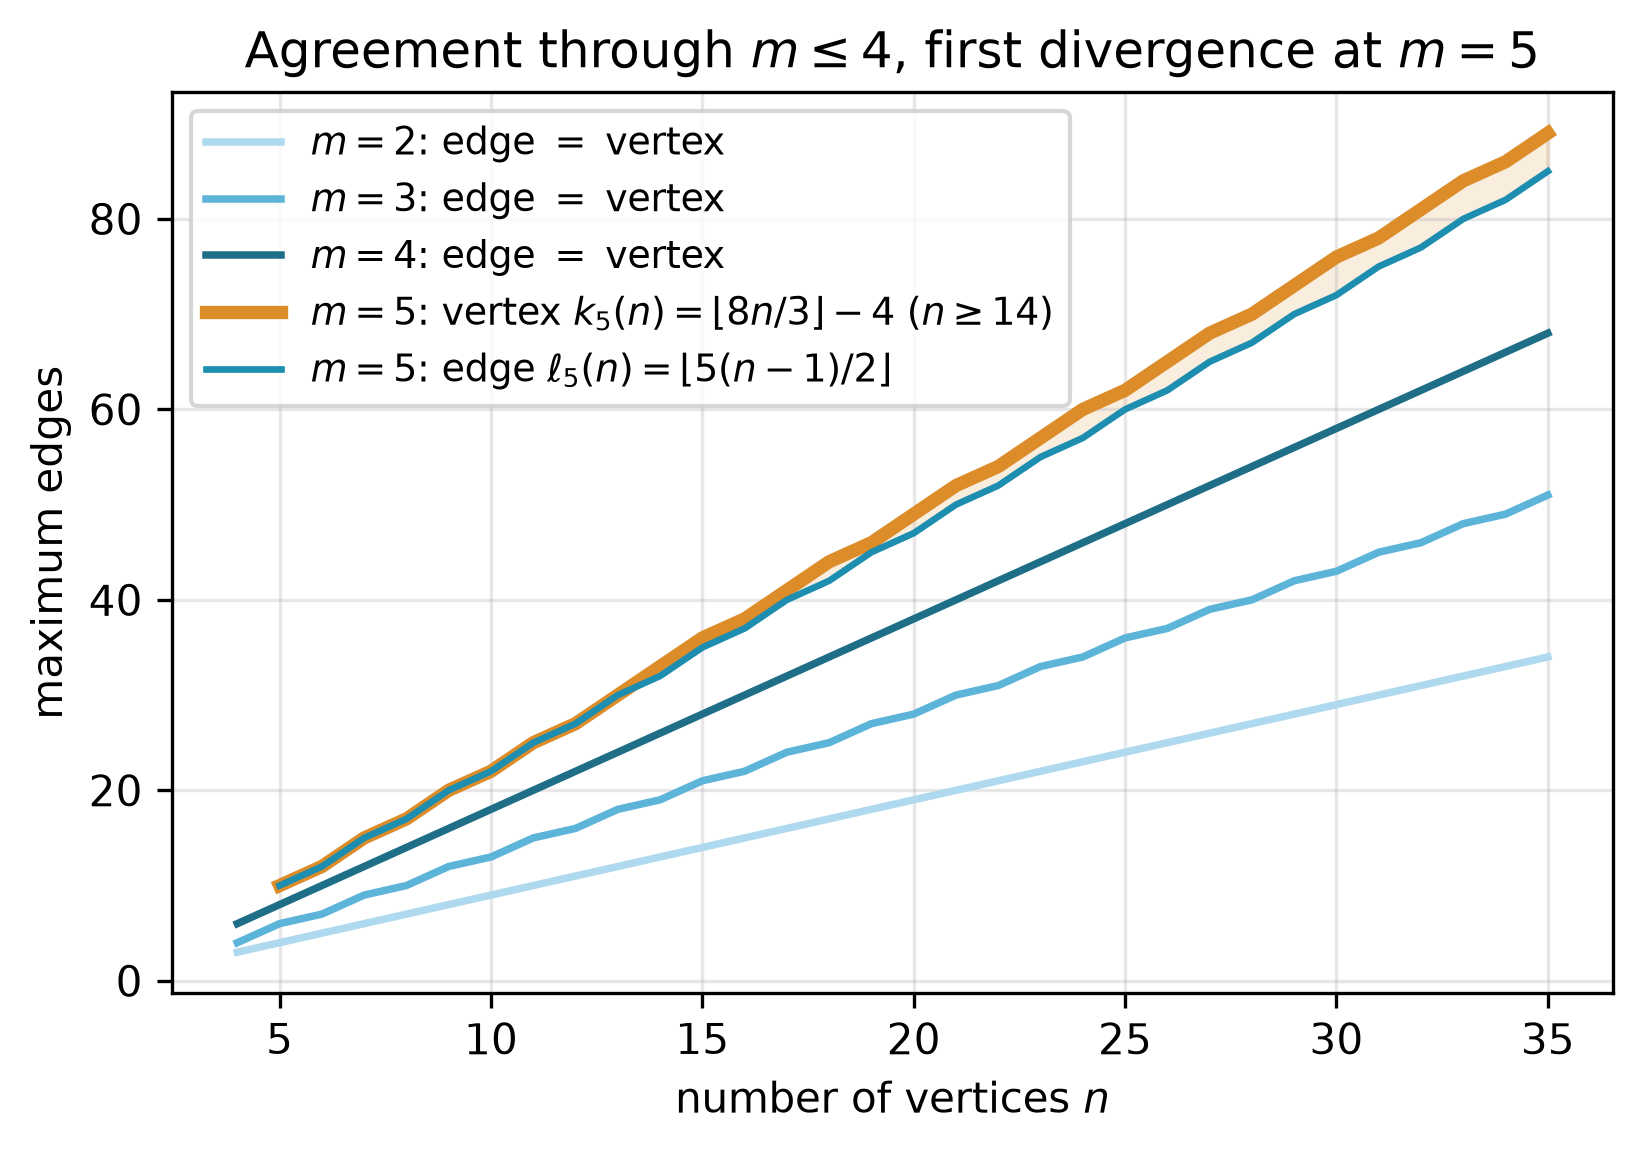
\includegraphics[width=\textwidth]{figures/edge_vertex_divergence.png}
    \caption{The edge and vertex extremal functions for $m = 2, 3, 4$ (blue shades, single curve per $m$ since they agree) and $m = 5$ (thin blue for edge, thick orange for vertex). The vertex function diverges from the edge function at $n = 14$ and grows faster thereafter.}
    \label{fig:divergence}
\end{figure}

\subsection{Directed graphs at the first threshold}

\begin{theorem}[Directed arc value at $m = 2$]\label{thm:dir-arc-m2-exact}
For simple digraphs,
\[
    \ell_2^{\mathrm{dir}}(n) = \max\!\left(2(n-1),\ \floorfrac{n^2}{4}\right).
\]
\end{theorem}

Two constructions attain the two terms (\Cref{fig:simple-digraph-m2}).
The bidirected star has $2(n-1)$ arcs.
The one-way complete bipartite digraph has all arcs from one half of the vertices to the other half, so it has $\floor{n^2/4}$ arcs.
In both, every ordered pair is joined by at most one directed path.
\Cref{sec:dir-constructions} gives the details.

For the upper bound we use a \emph{reachability skeleton}: a subdigraph in which $u$ can reach $v$ exactly when $u$ can reach $v$ in the whole digraph.
\Cref{lem:reach-skeleton} shows that there is always a skeleton with at most $M(n)=\max(2(n-1),\floor{n^2/4})$ arcs.
At $m=2$, an arc outside the skeleton would give a second route between its ends.
So a feasible digraph is its own skeleton.
This proves the bound for vertex separation, and so also for arc separation (\Cref{sec:dir-arc-m2}).

\begin{theorem}[Directed vertex value at $m = 2$]\label{thm:dir-vertex-m2-exact}
For simple digraphs, $k_2^{\mathrm{dir}}(n) = \ell_2^{\mathrm{dir}}(n)$.
\end{theorem}

\begin{figure}[ht]
\centering
\begin{tikzpicture}[>=Stealth, scale=1.0,
    smallleftvertex/.style={gvertex}, smallrightvertex/.style={gvsink},
    hubvertex/.style={gvhub}, leftvertex/.style={gvertex},
    arc/.style={gdir},
    carc/.style={gdir, vertexorange!80!black}]

  % --- left panel: the bidirected star at n = 7, hub plus six spokes = 12 arcs ---
  \begin{scope}[shift={(-5.4,1.0)}, scale=0.92]
    \node[hubvertex, minimum size=7mm] (h) at (0,0) {$h$};
    \foreach \i/\ang in {0/90, 1/150, 2/210, 3/270, 4/330, 5/30} {
      \node[leftvertex, minimum size=7mm] (v\i) at (\ang:2.2) {$\i$};
    }
    \foreach \i in {0,...,5} {
      \draw[arc] (h) to[bend left=13] (v\i);
      \draw[arc] (v\i) to[bend left=13] (h);
    }
  \end{scope}
  % --- right panel: B_{3,4} at n = 7, every A-to-B arc = 12 arcs ---
  \begin{scope}[on background layer]
    \node[draw=KULblauw1!25, fill=KULblauw1!6, rounded corners=10pt,
          fit={(0,-0.6) (0,2.6)}, inner sep=8pt, minimum width=12pt] {};
    \node[draw=vertexred!25, fill=vertexred!6, rounded corners=10pt,
          fit={(4,-0.6) (4,2.6)}, inner sep=8pt, minimum width=12pt] {};
  \end{scope}
  \foreach \i in {1,...,3} {
    \node[smallleftvertex]  (a\i) at (0, {2.0-1.0*(\i-1)}) {$a_{\i}$};
  }
  \foreach \j in {1,...,4} {
    \node[smallrightvertex] (b\j) at (4, {2.5-1.0*(\j-1)}) {$b_{\j}$};
  }
  \foreach \i in {1,...,3} {
    \foreach \j in {1,...,4} {
      \draw[arc] (a\i) -- (b\j);
    }
  }
  \node[font=\small] at (0,-1.3) {$A$};
  \node[font=\small] at (4,-1.3) {$B$};
\end{tikzpicture}
\caption{The two branches tie at $n=7$, where each holds $12$ arcs at $\lec^{\max}=1$. Left: the bidirected star, a hub joined to six spokes both ways, $2(n-1)=12$. Right: the one-directional complete bipartite digraph $B_{3,4}$, every arc from $A$ to $B$, $\floor{n^2/4}=12$.}
\label{fig:simple-digraph-m2}
\end{figure}

The star has more arcs for $n<7$, and the bipartite digraph has more for $n>7$.
So the directed value grows quadratically in $n$, while the undirected value grows linearly.
The reason is that all arcs can point the same way, so no route comes back.

\subsection{Undirected hypergraphs}

\begin{theorem}[Hypergraph edge bound]\label{prop:hyper-edge}
For $n\ge r\ge2$ and $m\ge2$, an $r$-uniform multihypergraph on $n$ vertices with $\lec^{\max}\le m-1$ has size at most $\floorfrac{(m-1)(n-1)}{r-1}$. There are simple hypergraphs attaining the bound when $m - 1 \le \binom{n-2}{r-2}$, and multihypergraphs attaining it when $(r-1) \mid n - 1$.
\end{theorem}

\Cref{app:proofs} proves the bound by induction on $n$: it cuts the hypergraph into two parts.
The star hypertree of \Cref{fig:hyper-star} attains the bound at $m=2$.
It has a hub joined to disjoint groups of $r-1$ vertices.
For $r\ge3$, simple hypergraphs attain the bound whenever $m-1\le\binom{n-2}{r-2}$ (\Cref{thm:simple-hyper-edge}).
So for $r\ge3$, unlike for graphs, repeated edges often do not help.
The condition says that there are enough different hyperedges.
When it fails, the simple value can be smaller.
For example, at $n=r=m=3$ there is only one possible hyperedge.
A simple hypergraph has one hyperedge, while a multihypergraph can have two copies of it (\Cref{rem:simple-hyper-necessary}).

\begin{figure}[ht]
\centering
\begin{tikzpicture}[scale=1.0,
   stn/.style={metrostop, minimum size=6mm},
   hub/.style={metrostop, minimum size=8.5mm, draw=vertexorange!90!black,
               fill=vertexorange!45, line width=1.4pt}]
  \coordinate (h) at (0,0);
  % two horizontal rows of four stations, the hub centred between them
  \coordinate (i1) at (-0.95, 1.3);  \coordinate (o1) at (-2.65, 1.3);
  \coordinate (i2) at ( 0.95, 1.3);  \coordinate (o2) at ( 2.65, 1.3);
  \coordinate (i3) at (-0.95,-1.3);  \coordinate (o3) at (-2.65,-1.3);
  \coordinate (i4) at ( 0.95,-1.3);  \coordinate (o4) at ( 2.65,-1.3);
  \begin{scope}[on background layer]
    % each hyperedge is one metro line: hub --(diagonal)-- inner --(horizontal)-- outer
    \draw[metro, metroA] (h) -- (i1) -- (o1);
    \draw[metro, metroB] (h) -- (i2) -- (o2);
    \draw[metro, metroC] (h) -- (i3) -- (o3);
    \draw[metro, metroD] (h) -- (i4) -- (o4);
  \end{scope}
  \foreach \p in {i1,o1,i2,o2,i3,o3,i4,o4} {\node[stn] at (\p) {};}
  \node[hub] at (h) {$h$};
\end{tikzpicture}
\caption{The $r=3$, $n=9$ star hypertree: four hyperedges meet only at the hub $h$, attaining $\floor{(n-1)/(r-1)}=4$ with $\lec^{\max}=1$.}
\label{fig:hyper-star}
\end{figure}

\begin{theorem}[Hypergraph vertex value at $m = 2$]\label{thm:hyper-vertex-m2}
For $r \ge 2$ and $n \ge 1$, the maximum number of hyperedges of an
$r$-uniform multihypergraph on $n$ vertices with $\kap^{\max} \le 1$ is
\[
    K_2^{(r)}(n) \;=\; \floorfrac{n-1}{r-1},
\]
attained by the star hypertree of \Cref{fig:hyper-star}, which is simple. In
particular $K_2^{(r)}(n) = k_2^{(r)}(n) = \ell_2^{(r)}(n)$: the vertex and edge
problems agree at $m = 2$ for every uniformity, and repeated hyperedges never
help.
\end{theorem}

\begin{theorem}[Hypergraph vertex value at $m = 3$]\label{thm:hyper-vertex-m3}
For $r \ge 2$ and $n\ge1$, every $r$-uniform multihypergraph on $n$ vertices with
$\kap^{\max} \le 2$ has at most $\floorfrac{2(n-1)}{r-1}$ hyperedges. For
$2 < r < n$, which is exactly the range where $2 \le \binom{n-2}{r-2}$, the bound
is attained by a simple hypergraph, so
\[
    k_3^{(r)}(n) \;=\; \floorfrac{2(n-1)}{r-1} \;=\; \ell_3^{(r)}(n).
\]
When $(r-1) \mid (n-1)$, a multihypergraph attains it, so then
$K_3^{(r)}(n) = \floor{2(n-1)/(r-1)}$
(\Cref{prop:hyper-vertex-lower-multi}).
\end{theorem}

Both proofs use the incidence graph (\Cref{sec:hyper-vertex-proof}).
At $m=3$ the proof bounds the number of independent cycles of the incidence graph.
We have no such bound for $m\ge4$.



For $r=2$ these results are about multigraphs.
They give $K_2(n)=n-1$, attained by trees, and $K_3(n)=2(n-1)$, attained by a tree with every edge doubled (\Cref{cor:multi-vertex-m3}).
For $m=5$ the vertex and edge values differ: the thickened theta of \Cref{sec:multi-vertex} gives $K_5(4)\ge14$, while $L_5(4)=12$.
For $m=4$ this is open.
\Cref{sec:multi-vertex} discusses larger $m$.

\subsection{Directed bounds beyond the first threshold}

\begin{theorem}[The quadratic bound with a linear error]\label{thm:dir-arc-linear-error}
For all $m \ge 2$ and $n \ge 2$, every simple digraph $D$ on $n$ vertices with $\lec^{\max}_D \le m-1$, or with $\kap^{\max}_D \le m-1$, satisfies
\[
    |A(D)| \;\le\; \floorfrac{n^2}{4} \;+\; 4(m-1)(n-1),
\]
so for each fixed $m$,
\[
    \ell_m^{\mathrm{dir}}(n) \;=\; \frac{n^2}{4} \;+\; \Theta_m(n) \quad\text{and}\quad k_m^{\mathrm{dir}}(n) \;=\; \frac{n^2}{4} \;+\; \Theta_m(n) \qquad (m\ge3)\text{.}
\]
\end{theorem}


\Cref{app:proofs} gives the proof. It counts routes of length two.
For an ordered pair $(u,v)$, the routes $u\to x\to v$ with different midpoints $x$, together with the arc $u\to v$, are disjoint.
So a feasible digraph has at most $m-1$ of them.
Summing over all pairs bounds $\sum_x d^+(x)\,d^-(x)$.
The proof is by induction on $n$.
If some vertex has total degree below $n/2$, we delete it and use the bound on $n-1$ vertices.
Otherwise every total degree is at least $n/2$, and the sum above makes $\sum_x \min(d^+(x),d^-(x))$ at most linear in $n$.
At every vertex we then delete its in-arcs or its out-arcs, whichever are fewer.
These deleted arcs give the linear term.
What remains has all arcs from one part to the other, so it has at most $\floor{n^2/4}$ arcs.
The routes of length two are also internally vertex-disjoint, so the same proof works for vertex separation.


\begin{theorem}[Directed multigraph value, every $n$ and $m$]\label{thm:dir-multi-full}
For all $n \ge 2$ and $m \ge 2$,
\[
    L_m^{\mathrm{dir}}(n) \;=\; (m-1)\,M(n), \qquad M(n) := \max\!\Bigl(2(n-1),\ \floorfrac{n^2}{4}\Bigr).
\]
\end{theorem}

The bound is attained in two ways: by a bidirected tree with every arc taken $m-1$ times, and by the one-way complete bipartite digraph with every arc taken $m-1$ times.
The proof works as follows.
Every feasible multigraph contains a small reachability skeleton.
Removing one copy of each skeleton arc lowers $\lec(u,v)$ by at least one for every pair with $\lec(u,v)>0$.
So $m-1$ such removals remove all arcs.
For $n\ge\max(8,2m)$ the bipartite construction is the only extremal multigraph, up to reversing all arcs (\Cref{thm:dir-multi-uniqueness}).

A directed hyperedge is \emph{forward} if it has one tail and $r-1$ heads, as above.

\begin{theorem}[The directed hypergraph constant]\label{thm:dir-hyper-constant}
Let $r \ge 2$ and $m \ge 2$. Every forward directed $r$-uniform multihypergraph
$\HH$ on $n \ge 2$ vertices with $\kap^{\max}_{\HH} \le m-1$ satisfies
\[
    |E(\HH)| \;\le\; \frac{m-1}{r-1}\floorfrac{n^2}{4} \;+\; 4(m-1)^2 (n-1).
\]

\end{theorem}

Since $\kap\le\lec$, the same bound holds when $\lec^{\max}_\HH\le m-1$. The construction of \Cref{prop:dir-hyper-first} has $(1+o(1))(m-1)n^2/(4(r-1))$ hyperedges, so the leading term is right.

\Cref{app:proofs} gives the proof.
It uses the \emph{shadow} digraph, which has an arc $u\to v$ when some hyperedge has tail $u$ and head $v$.
Each hyperedge gives $r-1$ arcs of the shadow, and each arc comes from at most $m-1$ hyperedges.
The route condition on the hypergraph limits the routes of length two in the shadow.
\Cref{lem:two-step-budget} then bounds the number of arcs of the shadow.

At $r=2$ this also covers directed multigraphs with vertex separation.
At $m=2$ no arc can be repeated, so $K_2^{\mathrm{dir}}(n)=\ell_2^{\mathrm{dir}}(n)$.
For fixed $m$, the extremal multigraphs of \Cref{thm:dir-multi-full} are feasible here too, since $\kap\le\lec$.
With \Cref{thm:dir-hyper-constant} at $r=2$ this gives $K_m^{\mathrm{dir}}(n)=(m-1)n^2/4+O_m(n)$ (\Cref{cor:dir-multi-incidence}).

\Cref{sec:status-simple-directed} compares this with a theorem of Huang and Lyu \cite{HuangLyu26}.
